\section{Cơ chế phát hiện leo thang đặc quyền của SyscallAD}
\label{sec:privesc}

Mục này nối mô-đun SyscallAD với ngữ cảnh đề tài: \emph{vì sao} một bộ phát hiện bất
thường syscall lại nắm bắt được hành vi leo thang đặc quyền, và \emph{đặc trưng nào}
mang tín hiệu đó.

\subsection{Ánh xạ syscall đặc quyền sang kỹ thuật leo thang}
Mọi con đường leo thang đặc quyền/thoát container đều phải gọi một số syscall
\emph{đặc quyền} mà khối lượng công việc lành tính hầu như không dùng. Bảng~%
\ref{tab:privesc-map} ánh xạ các syscall đặc quyền sang nhóm kỹ thuật tấn công và ví
dụ CVE; Hình~\ref{fig:privesc} minh họa trực quan.

\begin{table}[htbp]
  \centering
  \caption{Ánh xạ syscall đặc quyền $\to$ hành vi leo thang $\to$ kỹ thuật MITRE
           ATT\&CK / ví dụ CVE.}
  \label{tab:privesc-map}
  \small
  \begin{tabularx}{\linewidth}{@{}l >{\raggedright\arraybackslash}p{3.6cm} >{\raggedright\arraybackslash}X@{}}
    \toprule
    \textbf{Syscall} & \textbf{Hành vi} & \textbf{MITRE ATT\&CK / ví dụ} \\
    \midrule
    \texttt{ptrace}            & tiêm/điều khiển tiến trình khác & T1055 (Process Injection) \\
    \texttt{execve}+tải \texttt{.so} & lạm dụng nhị phân setuid & T1548; PwnKit (CVE-2021-4034) \\
    \texttt{setuid}/\texttt{capset} & đặt UID/capability đặc quyền & T1548 (Abuse Elevation Control) \\
    \texttt{unshare}/\texttt{setns} & thao tác namespace, vượt cô lập & T1611 (Escape to Host) \\
    \texttt{mount}/\texttt{pivot\_root} & gắn/đổi gốc hệ tệp & T1611; thoát qua host-path \\
    \texttt{openat}+\texttt{execve} & ghi đè \texttt{/proc/self/exe} & T1611; thoát \texttt{runc} (CVE-2019-5736) \\
    \texttt{init\_module}/\texttt{finit\_module} & nạp mô-đun nhân & T1014 (Rootkit) \\
    \texttt{bpf}               & nạp chương trình eBPF đặc quyền & T1068; lạm dụng \texttt{CAP\_BPF} \\
    \texttt{splice}            & ghi đè bộ đệm pipe & T1068; Dirty Pipe (CVE-2022-0847) \\
    \bottomrule
  \end{tabularx}

  \vspace{2pt}
  {\footnotesize\emph{Lưu ý:} (i) PwnKit và thoát \texttt{runc} \emph{không} tự gọi
  \texttt{setuid}; dấu vết của chúng là \texttt{execve} (vào \texttt{pkexec}/ghi đè
  \texttt{/proc/self/exe}) kèm tải thư viện/ghi tệp---bảng này gắn chúng với syscall
  \emph{thực sự xuất hiện trong vết}, nhất quán với Bảng~\ref{tab:bg-cve}. (ii) Một
  số khai thác dùng syscall ngoài bảng chữ cái syscall an ninh (ví dụ Dirty Pipe dùng cả
  \texttt{write}); khi đó SyscallAD vẫn bắt được nhờ bit hiện diện của syscall đặc
  quyền \emph{nằm trong} bảng chữ cái (\texttt{splice}).}
\end{table}

\begin{figure}[htbp]
  \centering
  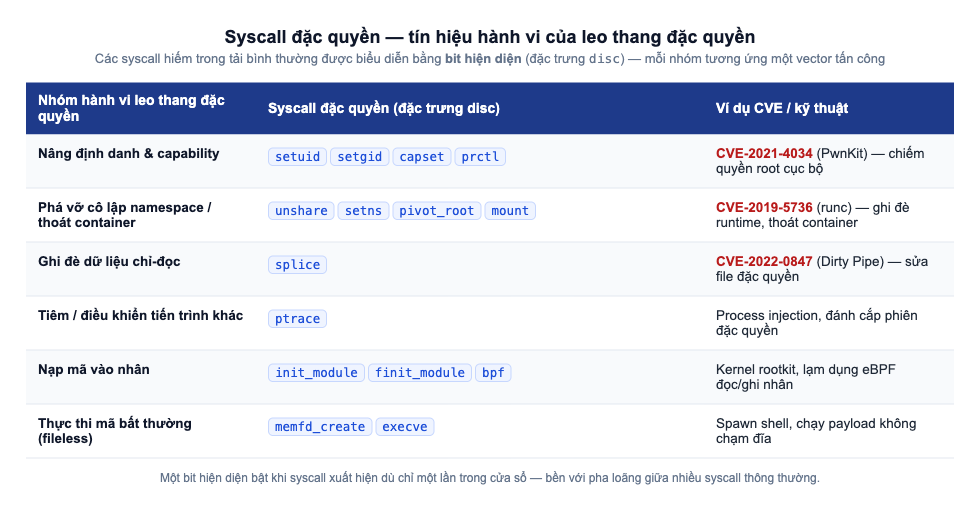
\includegraphics[width=\linewidth]{figures/privesc-syscalls}
  \caption{Ánh xạ các syscall đặc quyền (đặc trưng \texttt{disc}) sang nhóm hành vi
           leo thang đặc quyền và ví dụ CVE thực. Bit hiện diện của một syscall đặc
           quyền là tín hiệu phát hiện cốt lõi của SyscallAD.}
  \label{fig:privesc}
\end{figure}

\subsection{Vì sao đặc trưng \texttt{disc} là tín hiệu cốt lõi}
Trong một cửa sổ điển hình của khối lượng lành tính, các syscall đặc quyền gần như
không xuất hiện; còn trong cửa sổ chứa hành vi leo thang, chúng xuất hiện---dù chỉ
\emph{một lần}. Nếu dùng \emph{tần suất}, một \texttt{ptrace} đơn lẻ lẫn giữa 14 lời
gọi \texttt{openat} sẽ bị pha loãng tới mức gần như vô hình. SyscallAD vì thế mã hóa
các syscall đặc quyền hiếm bằng \textbf{bit hiện diện nhị phân} (đặc trưng
\texttt{disc}): bit bật ngay khi syscall xuất hiện, \emph{không} phụ thuộc mật độ.
Đây là lý do thiết kế khiến tấn công \emph{bền với pha loãng} và là cầu nối trực
tiếp giữa ``phát hiện bất thường'' và ``phát hiện leo thang đặc quyền''.

VAE củng cố tín hiệu này: vì chỉ học phân phối của cửa sổ \emph{bình thường} (nơi
các bit \texttt{disc} hầu như bằng 0), một cửa sổ có bit \texttt{disc} bật sẽ nằm xa
phân phối đã học và bị tái cấu trúc kém $\Rightarrow$ lỗi (điểm bất thường) cao.
iForest bổ trợ bằng cách cô lập tổ hợp syscall hiếm.

\subsection{Ví dụ minh họa một chuỗi tấn công}
Xét một chuỗi leo thang đặc quyền điển hình \texttt{clone} $\to$ \texttt{setuid}
$\to$ \texttt{execve} (kèm một \texttt{ptrace} dò xét). Khi đi qua đường ống:
\begin{enumerate}[leftmargin=1.8em]
  \item Cửa sổ chứa các lời gọi này bật các bit \texttt{disc} tương ứng
        (\texttt{setuid}, \texttt{ptrace}) và lệch ``chữ ký danh mục'' \texttt{cat}
        về phía nhóm \emph{process}/\emph{security}.
  \item Cửa sổ không khớp mẫu lành tính PrefixSpan $\Rightarrow$ đặc trưng
        \texttt{prefixspan} báo ``không khớp''.
  \item VAE trả lỗi tái cấu trúc cao; iForest cô lập cửa sổ ở độ sâu nông.
  \item Điểm hợp nhất $A(W_i)$ vượt ngưỡng $\Rightarrow$ cửa sổ bị gắn cờ.
\end{enumerate}
Ngược lại, một cửa sổ lành tính (ví dụ truy vấn cơ sở dữ liệu) chỉ gồm các syscall
phổ biến, khớp mẫu PrefixSpan và được VAE tái cấu trúc tốt $\Rightarrow$ điểm thấp,
không gắn cờ. Khoảng cách điểm giữa hai loại cửa sổ chính là cơ sở để đặt ngưỡng vận
hành (kết quả định lượng ở Mục~\ref{sec:results}).
